%!TEX root = index.tex
\section[Resultados]{Resultados}

\begin{frame}{Resultados}{Primeiros testes}
testes com R TODO
\end{frame}

\begin{frame}{Resultados}{Aquisição de dados}
\begin{center}
\begin{figure}[ht]
    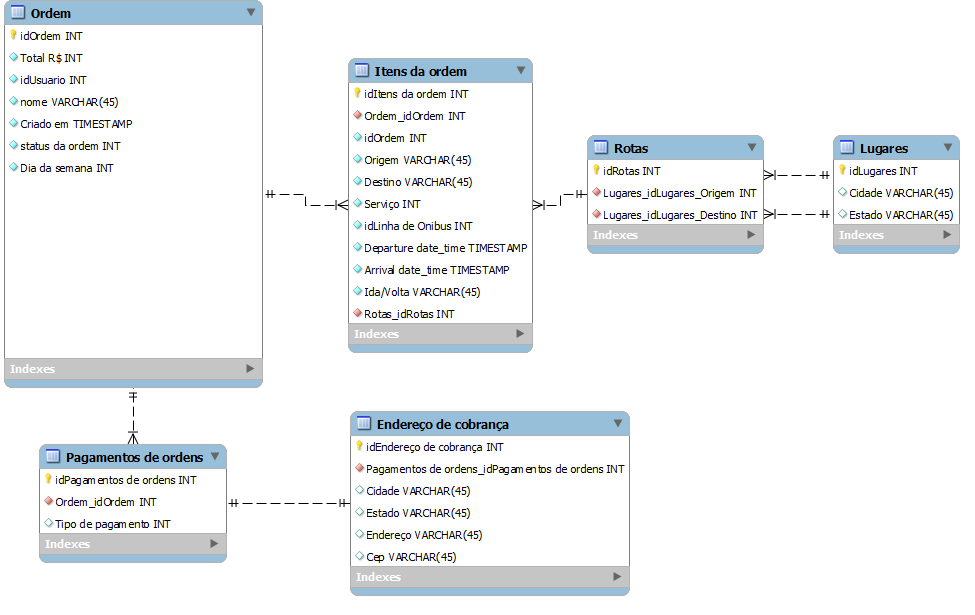
\includegraphics[width=0.8\textwidth]{../img/estrutura-banco-de-dados}
    \caption{Banco de dados de um e-commerce de passagens de ônibus}
    \label{fig:bd-clickbus}
\end{figure}
\end{center}
\end{frame}